
\section{Case Studies}

\begin{knitrout}
\definecolor{shadecolor}{rgb}{0.969, 0.969, 0.969}\color{fgcolor}\begin{kframe}
\begin{alltt}
\hlstd{opts_chunk}\hlopt{$}\hlkwd{set}\hlstd{(}\hlkwc{cache} \hlstd{=} \hlnum{TRUE}\hlstd{,} \hlkwc{autodep} \hlstd{=} \hlnum{TRUE}\hlstd{)}
\hlkwd{dep_auto}\hlstd{()}
\end{alltt}


{\ttfamily\noindent\color{warningcolor}{\#\# Warning in parse\_objects(paths[1L]): file cache/\_\_objects not found}}

{\ttfamily\noindent\color{warningcolor}{\#\# Warning in parse\_objects(paths[2L]): file cache/\_\_globals not found}}\end{kframe}
\end{knitrout}

In this section we demonstrate the use of the \pkg{sourceR} package using two example data sets. The first uses simulated data to demonstrate the general use case, with both time and location extensions for the model. The second is a specific case study using the the data described in the motivation section (Section \ref{sec:motivation}). The results (proportion of cases attributed to each source) are compared to the results from the Dutch, Modified Hald and Island models.

\subsection{Simulated data} \label{sim_study_section}

In this section, we provide a worked example using simulated data with multiple times and locations for source attribution data generated from the model in Section \ref{sec:model} (available in the \pkg{sourceR} data sets). There are two times (1, 2) and two locations (A, B) over which the human cases vary. The data expected by \code{saBayes} is in long format, with a column for the number of human cases, the number of positive samples for each source, and columns identifying the type, time and locations. Note, the source data is the same for all locations within a time. For this data, the source prevalences ($\pi_j$) are all set to be 1. If source prevalences are not provided, \code{saBayes} will automatically set them all to 1 (with a warning). The data must be in long format, with columns giving the number of human cases for each type, a column for each of the sources giving the number of positive samples for each type, and columns giving the time, location and type id's for each observation. 

\begin{table}
\caption{Minimum parameters required for the \code{saBayes} function.}
\label{table:HaldModelMinParams}
\begin{tabular}{p{4cm}p{11cm}}
\code{formula} & A formula object of the form $y\sim x1 + x2 + ... + xJ$, where $y$ is the name of the human cases column, and $x1, ...,xJ$ are the names of the source count columns in the data.\\
\code{time} & A formula object of the form $\sim t$, where $t$ is the name of the column containing the times in the data.\\
\code{location} & A formula object of the form $\sim l$, where $l$ is the name of the column containing the locations in the data.\\
\code{type} & A formula object of the form $\sim s$, where $s$ is the name of the column containing the (sub) types in the data.\\
\code{data} & Correctly formatted data.\\
\code{priors} & List with parameters for the prior distributions for each of the model parameters.\\
\code{n\_iter} & Specifies the number of iterations to run the algorithm for.\\
\code{likelihood_dist} & Specifies the likelihood distribution to be used for the human cases from each type. Must be one of \code{nbinom} or \code{pois}.\\
\end{tabular}
\end{table}

\begin{knitrout}
\definecolor{shadecolor}{rgb}{0.969, 0.969, 0.969}\color{fgcolor}\begin{kframe}
\begin{alltt}
\hlkwd{require}\hlstd{(sourceR)}
\hlkwd{set.seed}\hlstd{(}\hlnum{63164}\hlstd{)}
\hlkwd{data}\hlstd{(sim_SA)}
\hlkwd{data}\hlstd{(sim_SA_true)}

\hlcom{# Set priors}
\hlstd{priors} \hlkwb{<-} \hlkwd{list}\hlstd{(}\hlkwc{a} \hlstd{=} \hlnum{1}\hlstd{,} \hlkwc{r} \hlstd{=} \hlnum{1}\hlstd{,} \hlkwc{theta} \hlstd{=} \hlkwd{c}\hlstd{(}\hlnum{0.01}\hlstd{,} \hlnum{0.00001}\hlstd{))}

\hlcom{# Run model}
\hlstd{res} \hlkwb{<-} \hlkwd{saBayes}\hlstd{(}\hlkwc{formula} \hlstd{= Human} \hlopt{~} \hlstd{Source1} \hlopt{+} \hlstd{Source2} \hlopt{+} \hlstd{Source3} \hlopt{+} \hlstd{Source4} \hlopt{+} \hlstd{Source5,}
               \hlkwc{time} \hlstd{=} \hlopt{~}\hlstd{Time,} \hlkwc{location} \hlstd{=} \hlopt{~}\hlstd{Location,} \hlkwc{type} \hlstd{=} \hlopt{~}\hlstd{Type,}
               \hlkwc{data} \hlstd{= sim_SA}\hlopt{$}\hlstd{data,} \hlkwc{priors} \hlstd{= priors,}
               \hlkwc{alpha_conc} \hlstd{=} \hlnum{1}\hlstd{,} \hlkwc{prev} \hlstd{= sim_SA}\hlopt{$}\hlstd{prev,}
               \hlkwc{likelihood_dist} \hlstd{=} \hlstr{"pois"}\hlstd{,} \hlkwc{n_iter} \hlstd{=} \hlnum{1010}\hlstd{,}
               \hlkwc{mcmc_params} \hlstd{=} \hlkwd{list}\hlstd{(}\hlkwc{burn_in} \hlstd{=} \hlnum{20}\hlstd{,} \hlkwc{thin} \hlstd{=} \hlnum{1}\hlstd{))}
\end{alltt}
\end{kframe}
\end{knitrout}



The algorithm is run for 102,000 iterations using the \pkg{sourceR} command, with an initial burn in of 2000 iterations, followed by a further 100,000 iterations, of which every 100\textsuperscript{th} sample is saved. The acceptance rates for all parameters (except those updated using a Gibbs sampler) can be found in a list called \code{acceptance} in the output from \code{saBayes}. Trace and autocorrelation plots for the parameters (Figure~\ref{fig:trace_acf_sim_data_plots}) indicate that the Markov chain is mixing well and has converged, and that thinning by 100 is adequate. The posteriors are returned as nested lists for each parameter. The following R code demonstrates how to access the posteriors for a given source $a_{jtl}$ or type $q_i$ effects and a relative prevalence $r_{ijt}$.

\begin{knitrout}
\definecolor{shadecolor}{rgb}{0.969, 0.969, 0.969}\color{fgcolor}\begin{kframe}
\begin{alltt}
\hlcom{## Plot the marginal posterior for the source effect 2, at time 1, location A}
\hlkwd{plot}\hlstd{(res}\hlopt{$}\hlstd{posterior}\hlopt{$}\hlstd{a}\hlopt{$}\hlstd{time1}\hlopt{$}\hlstd{locationA[,}\hlstr{"Source3"}\hlstd{],} \hlkwc{type}\hlstd{=}\hlstr{"l"}\hlstd{)}
\hlcom{## Plot the marginal posterior for the type effect 21}
\hlkwd{plot}\hlstd{(res}\hlopt{$}\hlstd{posterior}\hlopt{$}\hlstd{q[,}\hlstr{"type21"}\hlstd{],} \hlkwc{type}\hlstd{=}\hlstr{"l"}\hlstd{)}
\hlcom{## Plot the marginal posterior for the relative prevalence of source effect 5, }
\hlcom{## type 17, at time 2}
\hlkwd{plot}\hlstd{(res}\hlopt{$}\hlstd{posterior}\hlopt{$}\hlstd{r}\hlopt{$}\hlstd{time2[}\hlstr{"type17"}\hlstd{,}\hlstr{"Source5"}\hlstd{,],} \hlkwc{type}\hlstd{=}\hlstr{"l"}\hlstd{)}
\end{alltt}
\end{kframe}
\end{knitrout}

\begin{knitrout}
\definecolor{shadecolor}{rgb}{0.969, 0.969, 0.969}\color{fgcolor}\begin{figure}

{\centering 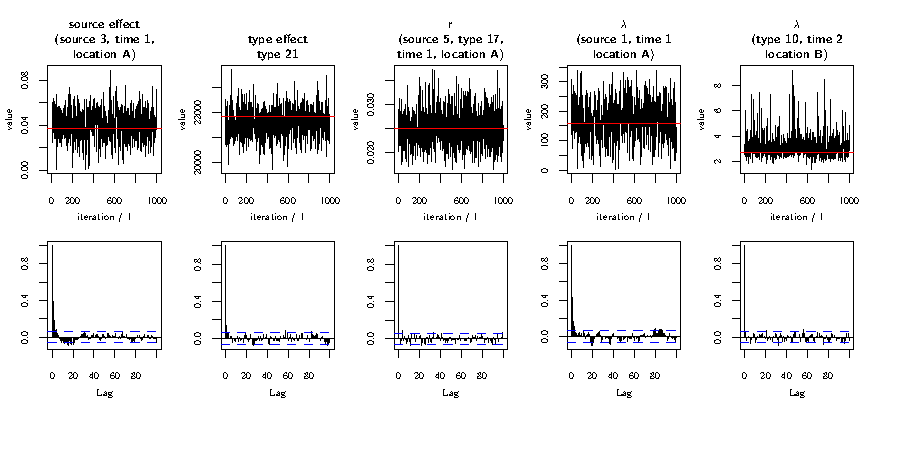
\includegraphics[width=\maxwidth]{figure/trace_acf_sim_data_plots-1} 

}

\caption[Trace and acf plots for a sample of the model parameters]{Trace and acf plots for a sample of the model parameters. True values of the parameters are shown in red.}\label{fig:trace_acf_sim_data_plots}
\end{figure}


\end{knitrout}

Medians and Chen-Shao highest posterior density credible intervals \citep{ChenShao99} can be obtained for each parameter using the \code{summary} command. 
%The credible intervals are Chen-Shao highest posterior density intervals which are the shortest possible Bayesian credible intervals, though 
%they can have high Monte Carlo error when  estimated directly from simulations via empirical shortest intervals \citep{LiuGelZhe15}. 

\begin{knitrout}
\definecolor{shadecolor}{rgb}{0.969, 0.969, 0.969}\color{fgcolor}\begin{kframe}
\begin{alltt}
\hlkwd{summary}\hlstd{(res,} \hlkwc{alpha} \hlstd{=} \hlnum{0.05}\hlstd{,} \hlkwc{thin} \hlstd{=} \hlnum{1}\hlstd{,} \hlkwc{burn_in} \hlstd{=} \hlnum{0}\hlstd{)}
\end{alltt}
\end{kframe}
\end{knitrout}

The data can be subsetted using the \code{subset_posterior} command.

\begin{knitrout}
\definecolor{shadecolor}{rgb}{0.969, 0.969, 0.969}\color{fgcolor}\begin{kframe}
\begin{alltt}
\hlkwd{subset_posterior}\hlstd{(res,} \hlkwc{params} \hlstd{=} \hlkwd{c}\hlstd{(}\hlstr{"a"}\hlstd{,} \hlstr{"li"}\hlstd{,} \hlstr{"q"}\hlstd{),}
                 \hlkwc{t} \hlstd{=} \hlstr{"1"}\hlstd{,} \hlkwc{l} \hlstd{=} \hlstr{"B"}\hlstd{,} \hlkwc{j} \hlstd{=} \hlkwd{c}\hlstd{(}\hlstr{"Source2"}\hlstd{,} \hlstr{"Source1"}\hlstd{),}
                 \hlkwc{i} \hlstd{=} \hlkwd{c}\hlstd{(}\hlstr{"47"}\hlstd{,} \hlstr{"10"}\hlstd{),} \hlkwc{iters} \hlstd{=} \hlkwd{c}\hlstd{(}\hlnum{3}\hlopt{:}\hlnum{10}\hlstd{))}
\end{alltt}
\end{kframe}
\end{knitrout}

Both the full posterior and a subset of the posterior (generated using \code{subset_posterior}) can be flattened into a data frame.

\begin{knitrout}
\definecolor{shadecolor}{rgb}{0.969, 0.969, 0.969}\color{fgcolor}\begin{kframe}
\begin{alltt}
\hlkwd{flatten}\hlstd{(res)}
\end{alltt}
\end{kframe}
\end{knitrout}

The marginal density plots of the proportion of cases attributed to each source at each time and location ($\lambda_{jtl}$) show that the true values (shown by a cross on the graph) are within the 
credible intervals (Figure~\ref{fig:sim_pois_lambdaj_plots}). The residual plots for $\lambda_{i}$ (Figure~
\ref{fig:lambda_i_residuals}) show that the model is fitting well. The heatmap shows the grouping of the type effects (Figure~\ref{fig:type_effect_heatmap}) computed using a dissimilarity matrix from the clustering output of the mcmc. The coloured bar under the dendrogram gives the correct grouping from the simulated data. This shows that 
all the types have been grouped correctly if the dendrogram is cut at the true number of groups (5).

\begin{knitrout}
\definecolor{shadecolor}{rgb}{0.969, 0.969, 0.969}\color{fgcolor}\begin{figure}

{\centering 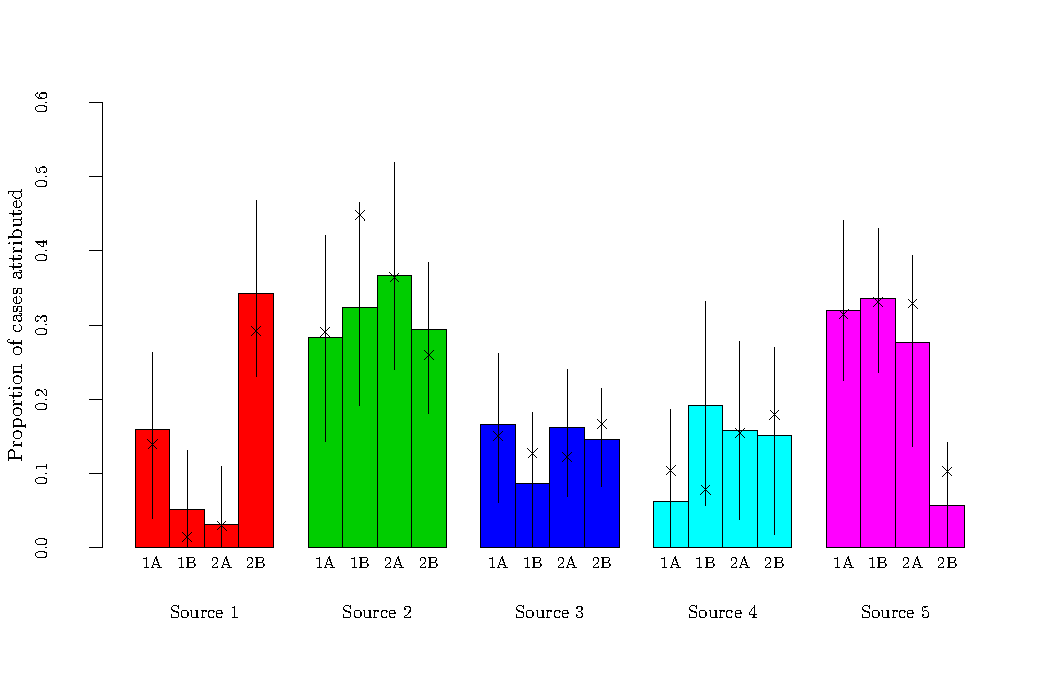
\includegraphics[width=\maxwidth]{figure/sim_pois_lambdaj_plots-1} 

}

\caption[Proportion of cases attributable to each source for each time (1, 2) and location (A, B) for simulated Poisson data]{Proportion of cases attributable to each source for each time (1, 2) and location (A, B) for simulated Poisson data. Error bars represent 95\% credible intervals. True $\lambda_j$ values are shown as crosses.}\label{fig:sim_pois_lambdaj_plots}
\end{figure}


\end{knitrout}


\begin{knitrout}
\definecolor{shadecolor}{rgb}{0.969, 0.969, 0.969}\color{fgcolor}\begin{figure}

{\centering 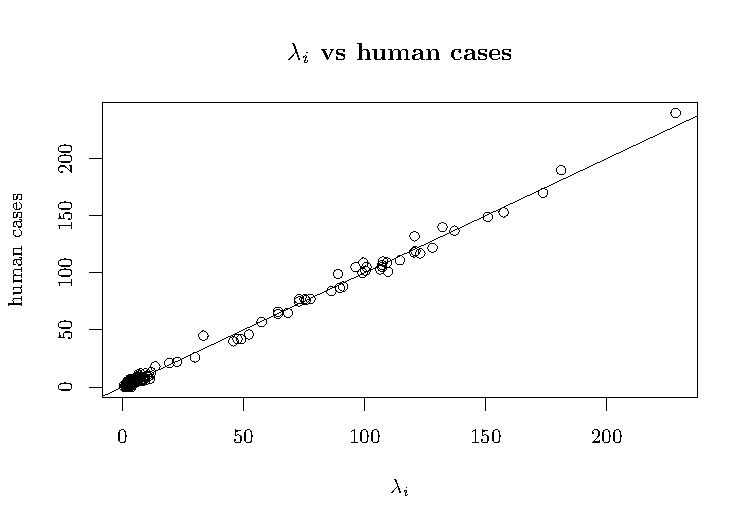
\includegraphics[width=\maxwidth]{figure/lambda_i_residuals-1} 

}

\caption[Residual plots]{Residual plots}\label{fig:lambda_i_residuals}
\end{figure}


\end{knitrout}


\begin{knitrout}
\definecolor{shadecolor}{rgb}{0.969, 0.969, 0.969}\color{fgcolor}\begin{figure}

{\centering 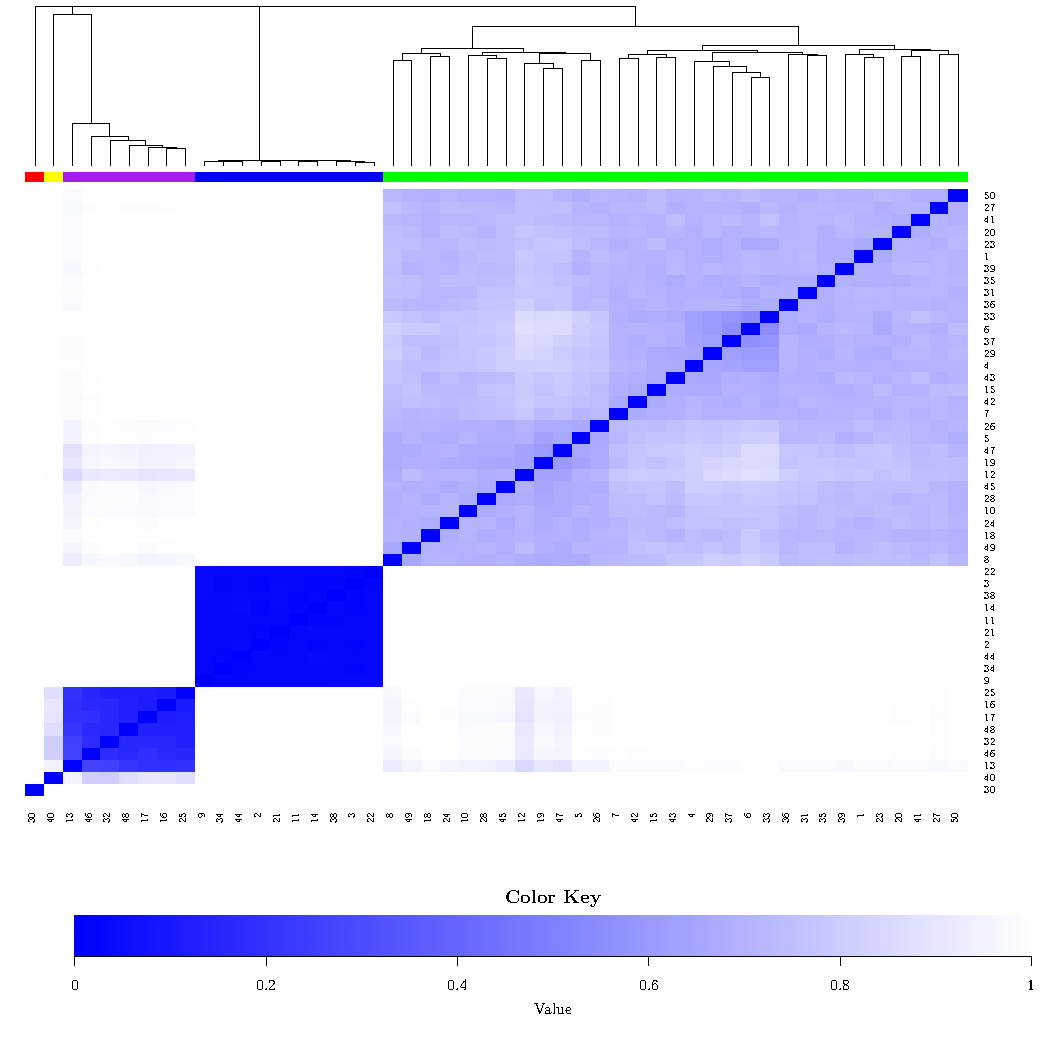
\includegraphics[width=\maxwidth]{figure/type_effect_heatmap-1} 

}

\caption[Heatmap showing the grouping of the type effects (q)]{Heatmap showing the grouping of the type effects (q)}\label{fig:type_effect_heatmap}
\end{figure}


\end{knitrout}

%%%%%%%%%%%%%%%%%%%%%%%%%%%%%%%%%%%%%%%%%%%%%%%%%%%%%%%%%%%%%%%%%%%%%%%%%%%%%%%%%%%%%%%%%%%%%%%%%
%%%%%%%%%%%%%%%%%%%%%%%%%%%%%%%%%%%%%%%%%%%%%%%%%%%%%%%%%%%%%%%%%%%%%%%%%%%%%%%%%%%%%%%%%%%%%%%%%
%%%%%%%%%%%%%%%%%%%%%%%%%%%%%%%%%%%%%%%%%%%%%%%%%%%%%%%%%%%%%%%%%%%%%%%%%%%%%%%%%%%%%%%%%%%%%%%%%

\subsection{Campylobacteriosis cases in the Manawatu (2005-2008)} \label{real_data_case_study_section}

In this section, we apply \pkg{sourceR} to the \code{campy} (campylobacteriosis) dataset from Manawatu, New Zealand, described in Section \ref{sec:motivation}.  We compare the results of our Bayesian non-parametric approach with results from the Modified Hald and Island models. Types which do not have any source cases need to be removed from the data set before running the analysis because there is no information to attribute human cases to a source if the subtype only occurs in humans.

\begin{knitrout}
\definecolor{shadecolor}{rgb}{0.969, 0.969, 0.969}\color{fgcolor}\begin{kframe}
\begin{alltt}
\hlkwd{data}\hlstd{(campy)}
\hlkwd{set.seed}\hlstd{(}\hlnum{59623}\hlstd{)}
\hlcom{# remove rows with no source cases as there is no information for}
\hlcom{# source attribution of human cases for these sources}
\hlstd{zero_rows} \hlkwb{<-} \hlkwd{which}\hlstd{(}\hlkwd{apply}\hlstd{(campy[,}\hlkwd{c}\hlstd{(}\hlnum{2} \hlopt{:} \hlnum{7}\hlstd{)],} \hlnum{1}\hlstd{, sum)} \hlopt{==} \hlnum{0}\hlstd{)}
\hlstd{campy} \hlkwb{<-} \hlstd{campy[}\hlopt{-}\hlstd{zero_rows,]}

\hlcom{# Set priors}
\hlstd{priors} \hlkwb{<-} \hlkwd{list}\hlstd{(}\hlkwc{a} \hlstd{=} \hlnum{1}\hlstd{,} \hlkwc{r} \hlstd{=} \hlnum{1}\hlstd{,} \hlkwc{theta} \hlstd{=} \hlkwd{c}\hlstd{(}\hlnum{0.01}\hlstd{,} \hlnum{0.00001}\hlstd{))}

\hlcom{# set prevalences}
\hlcom{# Number of samples  tested  for c. jejuni, for each source.}
\hlstd{tot_samples}\hlkwb{<-}\hlkwd{c}\hlstd{(}\hlnum{239}\hlstd{,} \hlnum{196}\hlstd{,} \hlnum{127}\hlstd{,} \hlnum{595}\hlstd{,} \hlnum{552}\hlstd{,} \hlnum{192} \hlopt{+} \hlnum{332}\hlstd{)}
\hlcom{# Number of samples positive for c. jejuni, for each source.}
\hlstd{pos_samples}\hlkwb{<-}\hlkwd{c}\hlstd{(}\hlnum{181}\hlstd{,} \hlnum{113}\hlstd{,} \hlnum{109}\hlstd{,} \hlnum{97}\hlstd{,} \hlnum{165}\hlstd{,} \hlnum{24} \hlopt{+} \hlnum{62}\hlstd{)}
\hlstd{prevs} \hlkwb{<-} \hlkwd{data.frame}\hlstd{(}\hlkwc{value} \hlstd{= pos_samples} \hlopt{/} \hlstd{tot_samples,}
                    \hlkwc{source_id} \hlstd{=} \hlkwd{colnames}\hlstd{(campy[,} \hlnum{2}\hlopt{:}\hlnum{7}\hlstd{]))}

\hlcom{# Run model}
\hlcom{# the model assumes one time and location if none are specified in saBayes}
\hlstd{res} \hlkwb{<-} \hlkwd{saBayes}\hlstd{(}\hlkwc{formula} \hlstd{= Human} \hlopt{~} \hlstd{ChickenA} \hlopt{+} \hlstd{ChickenB} \hlopt{+} \hlstd{ChickenC} \hlopt{+}
                 \hlstd{Bovine} \hlopt{+} \hlstd{Ovine} \hlopt{+} \hlstd{Environment,}
               \hlkwc{type} \hlstd{=} \hlopt{~}\hlstd{Type,} \hlkwc{data} \hlstd{= campy,} \hlkwc{priors} \hlstd{= priors,} \hlkwc{alpha_conc} \hlstd{=} \hlnum{1}\hlstd{,}
               \hlkwc{prev} \hlstd{= prevs,} \hlkwc{likelihood_dist} \hlstd{=} \hlstr{"pois"}\hlstd{,} \hlkwc{n_iter} \hlstd{=} \hlnum{1020}\hlstd{,}
               \hlkwc{mcmc_params} \hlstd{=} \hlkwd{list}\hlstd{(}\hlkwc{burn_in} \hlstd{=} \hlnum{20}\hlstd{,} \hlkwc{thin} \hlstd{=} \hlnum{1}\hlstd{))}
\end{alltt}
\end{kframe}
\end{knitrout}



Trace and autocorrelation plots for the parameters indicate that the Markov chain is mixing well and has converged, and that thinning by 500 is adequate for most of the parameters (Figure~
\ref{fig:trace_params_real}). The residual plots for the $\lambda_{i}$s (Figure~\ref{fig:lambda_i_residuals_real}) show that the model is fitting the data well. The proportion of cases attributed to each source ($\lambda_j$) using the new model can be compared to the previous models (Figure~\ref{fig:lambda_j_real}). The new 
model has very similar medians to the modified Hald and Island models. The credible intervals are much narrower than the modified Hald model, but still relatively wide compared to the Island model.
The heatmap and dendrogram of the type effects (Figure~
\ref{fig:type_effect_heatmap_real}) shows that there are 3 main groups of type effects. The violin plots (Figure~\ref{fig:type_effect_violinplots_real}) show that the largest group of types have very small type effects. These correspond to types that are observed in source samples, but no human cases. There is a group of 5 types which have very large type effects (including type 474 which is endemic to NZ and largely associated 
with poultry). Although the clustering was determined without reference to genetic relatedness of the types, three members of this group (subtypes 38, 48 and 474) are members of the same clonal complex (CC48) and therefore genetically closely related \citep{pubmlstCampy}. Subtype 52 was frequently placed in both the groups with the largest and middling type effects (as can be seen in Figure\ref{fig:type_effect_heatmap_real}, although overall it was attributed to the group with the largest type effects.

\begin{knitrout}
\definecolor{shadecolor}{rgb}{0.969, 0.969, 0.969}\color{fgcolor}\begin{figure}

{\centering 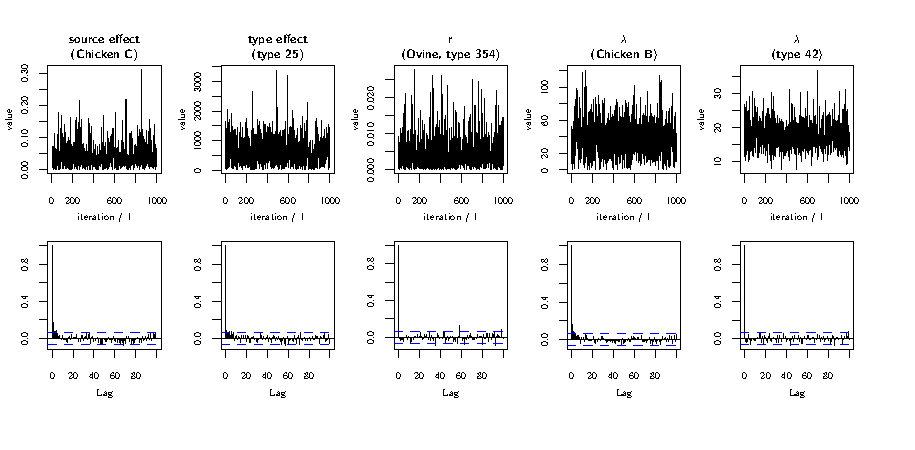
\includegraphics[width=\maxwidth]{figure/trace_params_real-1} 

}

\caption[Trace and acf plots for a sample of the model parameters (real data)]{Trace and acf plots for a sample of the model parameters (real data).}\label{fig:trace_params_real}
\end{figure}


\end{knitrout}

\begin{knitrout}
\definecolor{shadecolor}{rgb}{0.969, 0.969, 0.969}\color{fgcolor}\begin{figure}

{\centering 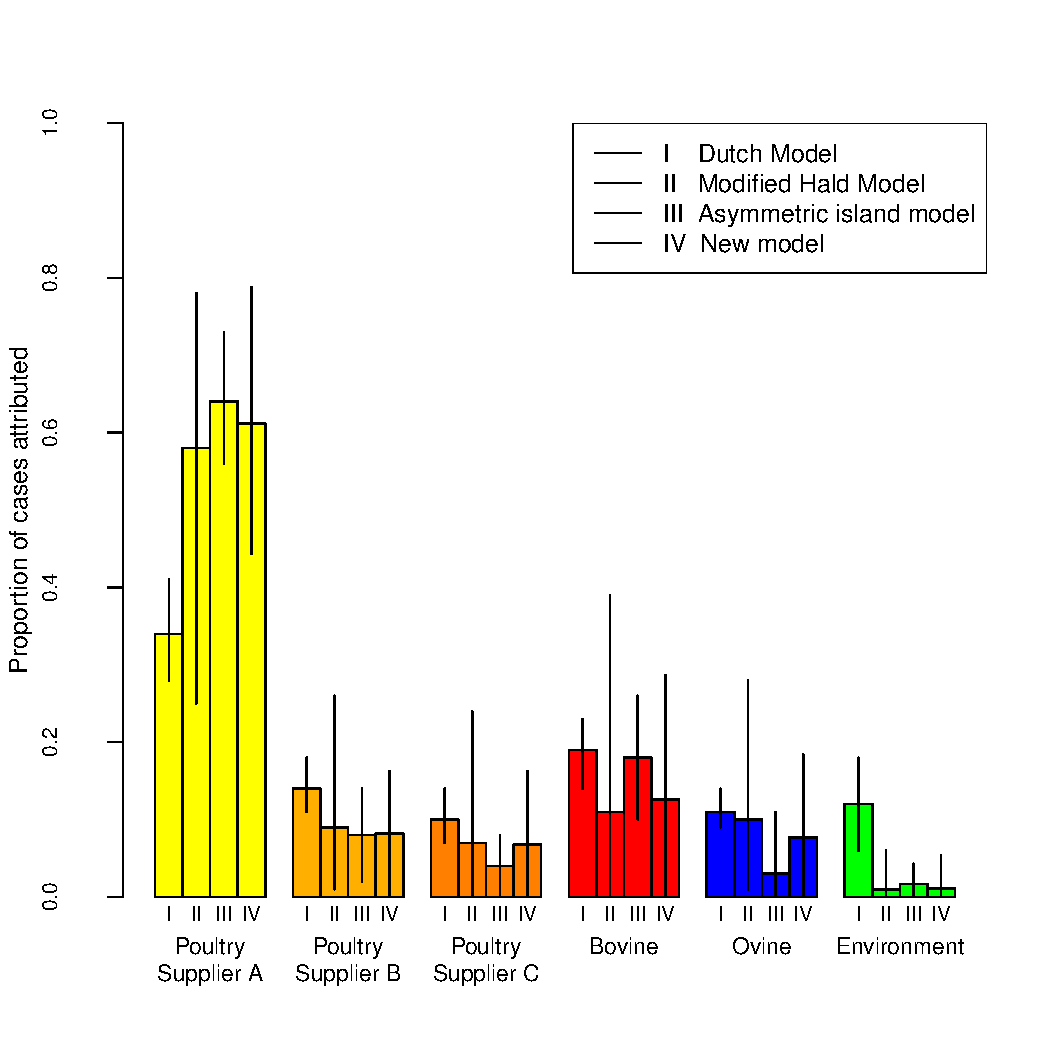
\includegraphics[width=\maxwidth]{figure/lambda_j_real-1} 

}

\caption[Proportion of human campylobacteriosis cases attributable to each source]{Proportion of human campylobacteriosis cases attributable to each source. Error bars represent 95\% confidence or credible intervals.}\label{fig:lambda_j_real}
\end{figure}


\end{knitrout}

\begin{knitrout}
\definecolor{shadecolor}{rgb}{0.969, 0.969, 0.969}\color{fgcolor}\begin{figure}

{\centering 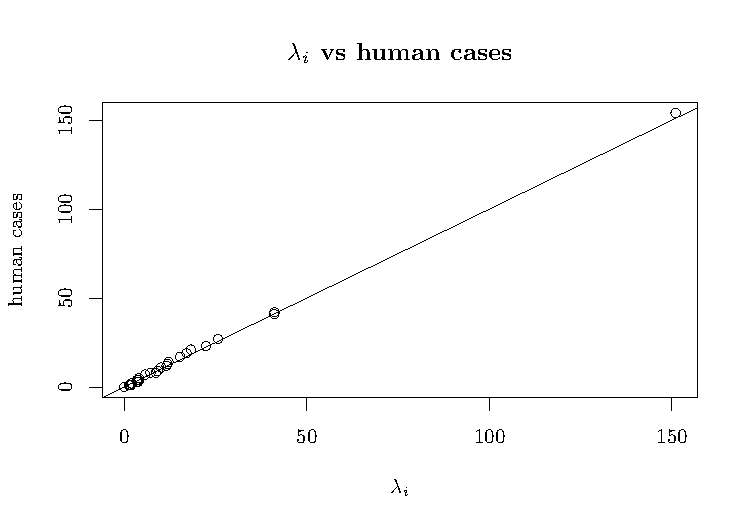
\includegraphics[width=\maxwidth]{figure/lambda_i_residuals_real-1} 

}

\caption[Residual plot]{Residual plot}\label{fig:lambda_i_residuals_real}
\end{figure}


\end{knitrout}

\begin{knitrout}
\definecolor{shadecolor}{rgb}{0.969, 0.969, 0.969}\color{fgcolor}\begin{kframe}


{\ttfamily\noindent\bfseries\color{errorcolor}{\#\# Error in `row.names<-.data.frame`(`*tmp*`, value = value): invalid 'row.names' length}}

{\ttfamily\noindent\bfseries\color{errorcolor}{\#\# Error in plot.new(): figure margins too large}}\end{kframe}\begin{figure}

{\centering 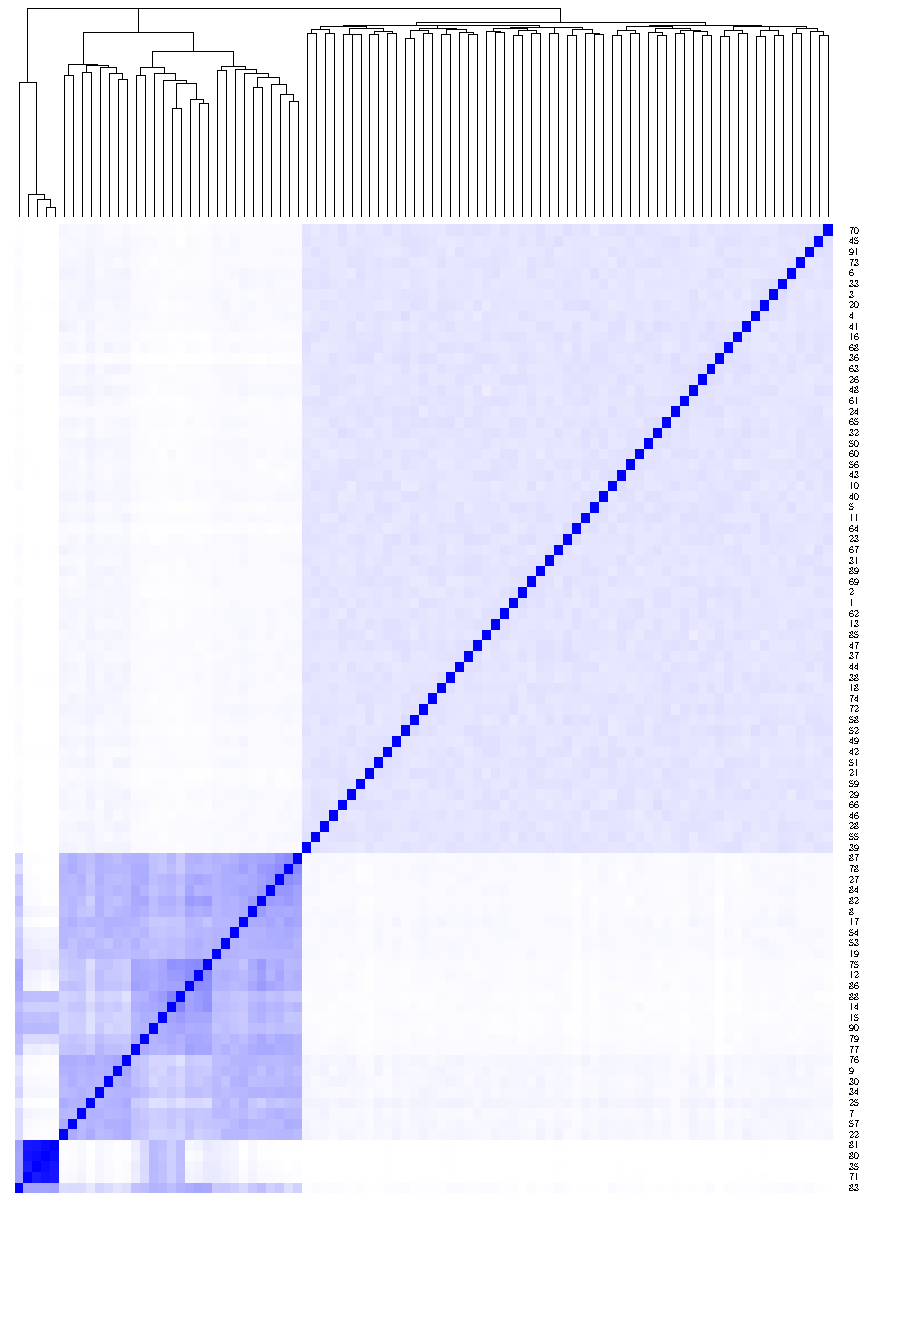
\includegraphics[width=\maxwidth]{figure/type_effect_heatmap_real-1} 

}

\caption[Heatmap showing the grouping of the type effects (q)]{Heatmap showing the grouping of the type effects (q)}\label{fig:type_effect_heatmap_real}
\end{figure}


\end{knitrout}


\begin{knitrout}
\definecolor{shadecolor}{rgb}{0.969, 0.969, 0.969}\color{fgcolor}\begin{figure}

{\centering 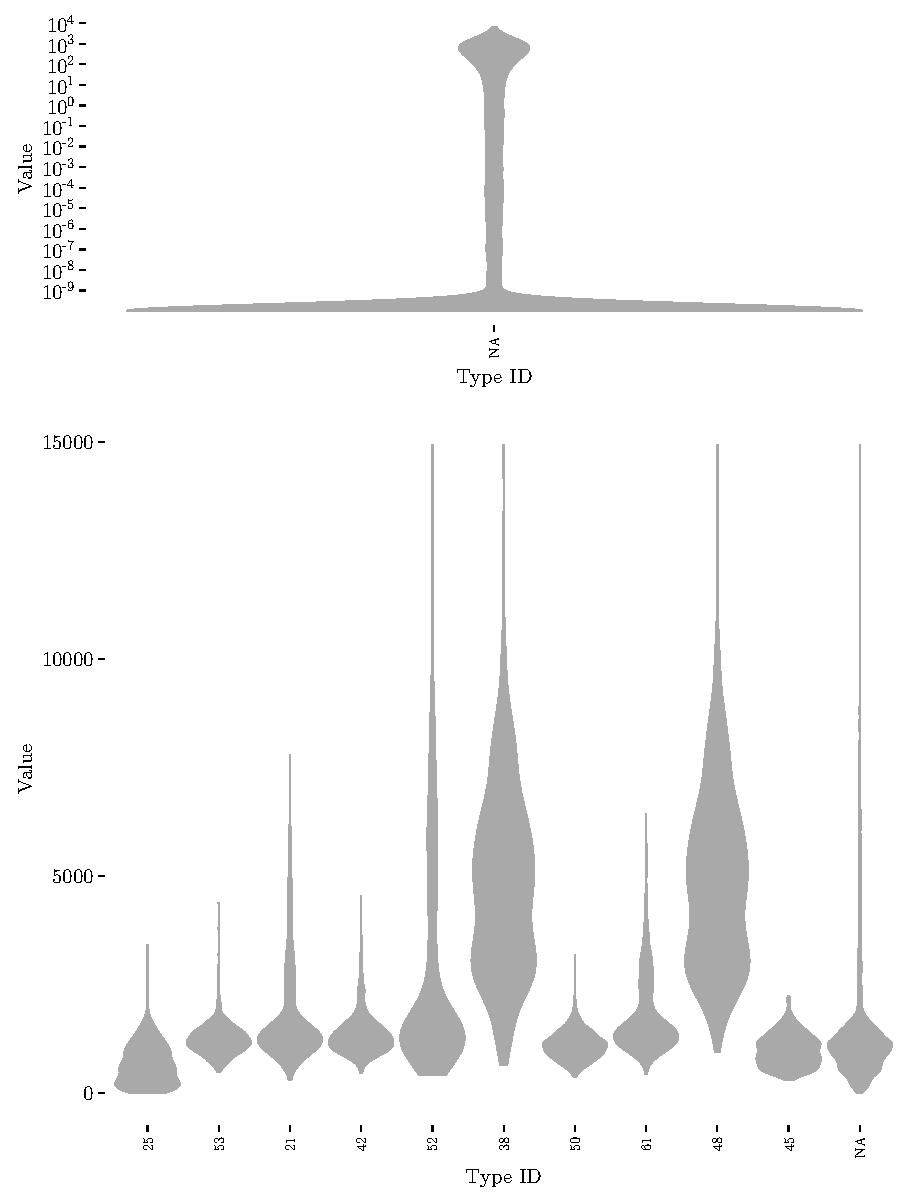
\includegraphics[width=\maxwidth]{figure/type_effect_boxplots_real1-1} 

}

\caption[Box plots of the type effects (q)]{Box plots of the type effects (q)}\label{fig:type_effect_boxplots_real1}
\end{figure}


\end{knitrout}

